\chapter{Vectorised Neural Networks}\label{ch:opencl}

Though the idea of Neural Networks is older than you might think (refer Chapter \ref{ch:intro}), it is only recently that the techniques started to yield the impressive results that have quickly become synonymous with its name. The reasons for this are myriad, but a large factor was the initial one: the march of technology is catching up with the requirements needed by complex neural networks. To utilise this increase in computing power, various optimisations have been developed for representing neural networks, and an important concept in this is parallelisation. By its very design as a great number of very simple entities, a neural network is a good fit for exploiting modern graphics cards, which consist of hundreds or thousands of cores able to perform a small number of relatively simple tasks. The modern GPU is optimised for matrix and vector calculations, because this is how 3D-graphics are represented. In this chapter we see how neural networks can be represented using basic linear algebra (the area of math concerned with vectors and matrices) to enable us to utilise this vast amount of parallel computing power.

\section{Neural Networks as Matrix-products}\label{sec:nnmp}
We can use the notation and intuitions described above to represent neural networks in a way that can be parallelised. The activation of each layer, whether it is input, output or hidden, is represented by a vector. Weights are represented in matrices, which transform the activation of a layer $a\i L$ to the activation of the next $a^{(L+1)}$ via matrix multiplication. Bias can be represented in multiple ways, but either requires an additional vector or an extra column in each weight-matrix. Gradient descent is used to train the network, like in the object-oriented representation described in Section~\ref{sec:gradient}.

\paragraph{Perceptron}
We start by examining a simple example, a single perceptron:
  \begin{center}
    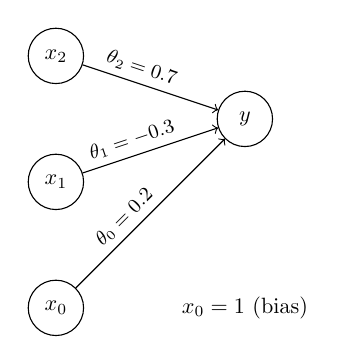
\begin{tikzpicture}[scale=0.8, transform shape]
      \node (x0)[circle, draw, minimum width=25pt] at (0, -2) {$x_0$};
      \node (x1)[circle, draw, minimum width=25pt] at (0, 0) {$x_1$};
      \node (x2)[circle, draw, minimum width=25pt] at (0, 2) {$x_2$};
      \node (y)[circle, draw, minimum width=25pt] at (3, 1) {$y$};
      \node (bias)[] at (3,-2) {$x_0 = 1$ (bias)};
      \draw[->] (x0) -- (y) node[pos=0.4,sloped,above] {\small $\theta_0 = 0.2$};
      \draw[->] (x1) -- (y) node[pos=0.4,sloped,above] {\small $\theta_1 = -0.3$};
      \draw[->] (x2) -- (y) node[pos=0.4,sloped,above] {\small $\theta_2 = 0.7$};
    \end{tikzpicture}
  \end{center}

Instead of considering each input $x_n$ and each weight $\theta_n$ as a separate value, we store them in two vectors $\vec x$ and $\vec\theta$. Normally, we use the matrix $\Theta$ to store the weights between two layers, where each column matches a node in the domain ($a\i L$, the input of the transformation) and each row matches a node in the co-domain ($a^{(L+1)}$, the output of the transformation). In this case, we have a single node in the co-domain, so the weight-matrix consists of a single row: a vector.

By taking the inner product of the input vector $\vec x$ and the weight vector $\vec \theta$, we can use a single operation to multiply each input value with its associated weight, and sum the result. So $y = \sigma(\theta_1x_1 + \theta_2x_2)$ becomes $y = \sigma\inprod{\theta}{x}$\footnote{Remember, $\sigma$ represents the \textit{sigmoid activation function}, as introduced in Section \ref{sec:neuron_revisted}.}.

Note that the bias is, in this case, added as a column to the weight matrix (or rather, in this simple example, a single value added to the weight matrix). This value is typically added as column $0$, which in this vector example means $\theta_0$. Furthermore, each input and activation layer is prepended\footnote{So, $\begin{bmatrix}x_1 & x_2\end{bmatrix}$ becomes $\begin{bmatrix}1 & x_1 & x_2\end{bmatrix} $. We can write this as $\vec a \leftarrow \begin{bmatrix}1 & \vec a\end{bmatrix}$.} with a $0$-index element, which will alway be $1$ (as $1 \times \theta_0 = \theta_0$, the bias). Thus, the expansion of our inner product including the bias is $y = \sigma(\theta_0x_0 + \theta_1x_1 + \theta_2x_2)$. In a later example, we will see another way to represent the bias using a separate vector.

\paragraph{Hidden Layer}
We now consider a more complicated network, by adding a single hidden layer consisting of $4$ neurons.

  \vspace{3mm}
  \begin{center}
    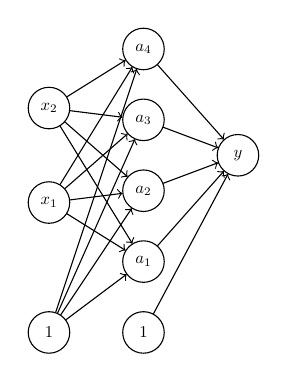
\begin{tikzpicture}[scale=0.6, transform shape]
      \node (x0)[circle, draw, minimum width=25pt] at (0, -3.75) {$1$};
      \node (x1)[circle, draw, minimum width=25pt] at (0, -1) {$x_1$};
      \node (x2)[circle, draw, minimum width=25pt] at (0, 1) {$x_2$};
      \node (a1)[circle, draw, minimum width=25pt] at (2, -2.25) {$a_1$};
      \node (a2)[circle, draw, minimum width=25pt] at (2, -0.75) {$a_2$};
      \node (a3)[circle, draw, minimum width=25pt] at (2, 0.75) {$a_3$};
      \node (a4)[circle, draw, minimum width=25pt] at (2, 2.25) {$a_4$};
      \node (a0)[circle, draw, minimum width=25pt] at (2, -3.75) {$1$};
      \node (y)[circle, draw, minimum width=25pt] at (4, 0) {$y$};
      \draw[->] (x0) -- (a1) [] {};
      \draw[->] (x0) -- (a2) [] {};
      \draw[->] (x0) -- (a3) [] {};
      \draw[->] (x0) -- (a4) [] {};
      \draw[->] (x1) -- (a1) [] {};
      \draw[->] (x1) -- (a2) [] {};
      \draw[->] (x1) -- (a3) [] {};
      \draw[->] (x1) -- (a4) [] {};
      \draw[->] (x2) -- (a1) [] {};
      \draw[->] (x2) -- (a2) [] {};
      \draw[->] (x2) -- (a3) [] {};
      \draw[->] (x2) -- (a4) [] {};
      \draw[->] (a1) -- (y) [] {};
      \draw[->] (a2) -- (y) [] {};
      \draw[->] (a3) -- (y) [] {};
      \draw[->] (a4) -- (y) [] {};
      \draw[->] (a0) -- (y) [] {};
    \end{tikzpicture}
\end{center}

We can calculate $a_1$ as $\inprod{x}{{\theta\i1}}$, $a_2$ as $\inprod{x}{{\theta\i2}}$, et cetera. But, as we have seen, we can do an entire series of inner products as a single operation using the matrix product. Multiplying $A\vec b =c$, each element $\vec c_y$ in $\vec c$ is calculated by $\inprod{A_{x,*}}{\vec b_y}$. We can use this to our advantage, and stack every weight vector $\vec{\theta\i n}$ for every neuron $a_n$ into a weight matrix $\Theta$. Multiplying this with our input vector $\vec x$ results in a new vector $\vec a$, consisting of all activation values in the succeeding layer.

$$\Theta\i1 = \begin{bmatrix}- & \vec{\theta^1} & - \\ - & \vec{\theta^2} & - \\ - & \vec{\theta^3} & - \\ - & \vec{\theta^4} & -\end{bmatrix}, \quad \vec{a} = \sigma(\Theta\i1\vec{x})$$

The entire picture now looks like this:

  \begin{minipage}{0.3\textwidth} \begin{center}
    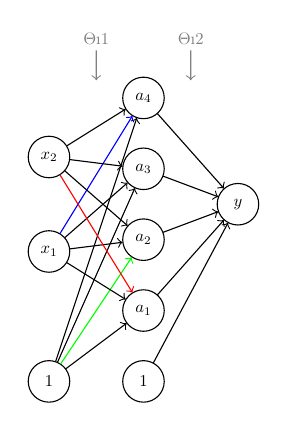
\begin{tikzpicture}[scale=0.6, transform shape]
      \node (l1)[] at (1,3.5) {\color{gray} $\Theta\i1$};
      \node (l2)[] at (3,3.5) {\color{gray} $\Theta\i2$};
      \node (t1)[] at (1,2.5) {};
      \node (t2)[] at (3,2.5) {};
      \draw[gray, ->] (l1) -- (t1) [] {};
      \draw[gray, ->] (l2) -- (t2) [] {};
      \node (x0)[circle, draw, minimum width=25pt] at (0, -3.75) {$1$};
      \node (x1)[circle, draw, minimum width=25pt] at (0, -1) {$x_1$};
      \node (x2)[circle, draw, minimum width=25pt] at (0, 1) {$x_2$};
      \node (a1)[circle, draw, minimum width=25pt] at (2, -2.25) {$a_1$};
      \node (a2)[circle, draw, minimum width=25pt] at (2, -0.75) {$a_2$};
      \node (a3)[circle, draw, minimum width=25pt] at (2, 0.75) {$a_3$};
      \node (a4)[circle, draw, minimum width=25pt] at (2, 2.25) {$a_4$};
      \node (a0)[circle, draw, minimum width=25pt] at (2, -3.75) {$1$};
      \node (y)[circle, draw, minimum width=25pt] at (4, 0) {$y$};
      \draw[->] (x0) -- (a1) [] {};
      \draw[green, ->] (x0) -- (a2) [] {};
      \draw[->] (x0) -- (a3) [] {};
      \draw[->] (x0) -- (a4) [] {};
      \draw[->] (x1) -- (a1) [] {};
      \draw[->] (x1) -- (a2) [] {};
      \draw[->] (x1) -- (a3) [] {};
      \draw[blue, ->] (x1) -- (a4) [] {};
      \draw[red, ->] (x2) -- (a1) [] {};
      \draw[->] (x2) -- (a2) [] {};
      \draw[->] (x2) -- (a3) [] {};
      \draw[->] (x2) -- (a4) [] {};
      \draw[->] (a1) -- (y) [] {};
      \draw[->] (a2) -- (y) [] {};
      \draw[->] (a3) -- (y) [] {};
      \draw[->] (a4) -- (y) [] {};
      \draw[->] (a0) -- (y) [] {};
    \end{tikzpicture}
  \end{center} \end{minipage}\begin{minipage}{0.7\textwidth}
    $$\Theta\i1 = \begin{bmatrix}0.1 & -0.2 & \color{red} -0.3 \\ \color{green} 0.4 & -0.5 & 0.6 \\ -0.7 & 0.8 & 0.9 \\ -0.1 & \color{blue}0.2 & 0.3\end{bmatrix}$$ $$\Theta\i2 = \begin{bmatrix}0.1 & 0.1 & 0.2 & 0.3 & 0.5\end{bmatrix}$$
  \end{minipage}\mbox{}\\[4mm]

    Each value in $\Theta\i 1$ matches a weight between the input and hidden layer; $\Theta\i1_{ij}$ represents the weight from $x_j$ to $a_i$. In this case, rows count from $1$, columns count from $0$ with column $0$ representing the bias. Each value in $\Theta\i 2$ matches a weight between the hidden layer and the output. In this case, it could have been represented by a vector because the output value $y$ is a scalar, but to avoid mixing and matching lowercase and uppercase Greek letters we keep every weight a matrix for now. Calculating $y$ from $\vec x$, $\Theta\i 1$, and $\Theta\i 2$ looks like this:

  $$\vec{a} = \sigma(\Theta\i1\vec{x}), \quad \vec{a^\prime} = \begin{bmatrix} 1 & \vec{a}\end{bmatrix}, \quad y = \sigma(\Theta\i2\vec{a^\prime})$$

  $$y = \sigma(\Theta\i2\vec{\begin{bmatrix} 1 & \sigma(\Theta\i1\vec{x})\end{bmatrix}})$$

\paragraph{Bias}
  So far, we have been representing the bias for each layer using an extra weight, which gets multiplied by $1$ for each neuron in the layer. An alternative way of representing the bias is as a separate vector, to be added after the matrix multiplication. Using the same sample as above, we can also represent the network as shown below. This time, both rows and columns count from 1 as there is no bias column $0$.

  \begin{minipage}{0.4\textwidth} \begin{center}
    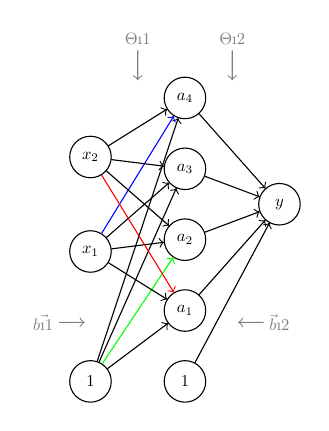
\begin{tikzpicture}[scale=0.6, transform shape]
      \node (l1)[] at (1,3.5) {\color{gray} $\Theta\i1$};
      \node (l2)[] at (3,3.5) {\color{gray} $\Theta\i2$};
      \node (l3)[] at (-1, -2.5) {\color{gray} $\vec{b\i1}$};
      \node (l4)[] at (4, -2.5) {\color{gray} $\vec b\i2$};
      \node (t1)[] at (1,2.5) {};
      \node (t2)[] at (3,2.5) {};
      \node (t3)[] at (0,-2.5) {};
      \node (t4)[] at (3,-2.5) {};
      \draw[gray, ->] (l1) -- (t1) [] {};
      \draw[gray, ->] (l2) -- (t2) [] {};
      \draw[gray, ->] (l3) -- (t3) [] {};
      \draw[gray, ->] (l4) -- (t4) [] {};
      \node (x0)[circle, draw, minimum width=25pt] at (0, -3.75) {$1$};
      \node (x1)[circle, draw, minimum width=25pt] at (0, -1) {$x_1$};
      \node (x2)[circle, draw, minimum width=25pt] at (0, 1) {$x_2$};
      \node (a1)[circle, draw, minimum width=25pt] at (2, -2.25) {$a_1$};
      \node (a2)[circle, draw, minimum width=25pt] at (2, -0.75) {$a_2$};
      \node (a3)[circle, draw, minimum width=25pt] at (2, 0.75) {$a_3$};
      \node (a4)[circle, draw, minimum width=25pt] at (2, 2.25) {$a_4$};
      \node (a0)[circle, draw, minimum width=25pt] at (2, -3.75) {$1$};
      \node (y)[circle, draw, minimum width=25pt] at (4, 0) {$y$};
      \draw[->] (x0) -- (a1) [] {};
      \draw[green, ->] (x0) -- (a2) [] {};
      \draw[->] (x0) -- (a3) [] {};
      \draw[->] (x0) -- (a4) [] {};
      \draw[->] (x1) -- (a1) [] {};
      \draw[->] (x1) -- (a2) [] {};
      \draw[->] (x1) -- (a3) [] {};
      \draw[blue, ->] (x1) -- (a4) [] {};
      \draw[red, ->] (x2) -- (a1) [] {};
      \draw[->] (x2) -- (a2) [] {};
      \draw[->] (x2) -- (a3) [] {};
      \draw[->] (x2) -- (a4) [] {};
      \draw[->] (a1) -- (y) [] {};
      \draw[->] (a2) -- (y) [] {};
      \draw[->] (a3) -- (y) [] {};
      \draw[->] (a4) -- (y) [] {};
      \draw[->] (a0) -- (y) [] {};
    \end{tikzpicture}
  \end{center} \end{minipage}\hspace{1mm}\begin{minipage}{0.55\textwidth} \small
    $$\Theta\i1 = \begin{bmatrix} -0.2 & \color{red} -0.3 \\ -0.5 & 0.6 \\ 0.8 & 0.9 \\ \color{blue}0.2 & 0.3\end{bmatrix},
    \vec{b\i1} = \begin{bmatrix}0.1 \\ \color{green} 0.4 \\ -0.7 \\ -0.1\end{bmatrix}$$\\
      $$\Theta\i2 = \begin{bmatrix}0.1 & 0.2 & 0.3 & 0.5\end{bmatrix}, \quad \vec b^{(2)} = \begin{bmatrix}0.1 \end{bmatrix}$$
  \end{minipage}\mbox{}\\[4mm]
  $$\vec{a} = \sigma(\Theta\i1\vec{x} + \vec{b\i1}), \quad y = \sigma(\Theta\i2\vec{a}+\vec b\i2)$$

  $$y = \sigma(\Theta\i2\sigma(\Theta\i1\vec{x} + \vec{b\i1})+\vec b\i2)$$\\[-4mm]

  Notice that we have written $\vec b\i 2$ as a $1$-element vector instead of a scalar, just as we write the single row matrix $\Theta\i 2$ as a matrix instead of a vector.\\

\begin{exercise}[Bias Representation]\mbox{}\\
  Confirm the equivalence of both bias representations by calculating the results in both instances.\\
  \textbf{Bonus:} Prove both bias representations are the same.
\end{exercise}

\def\Item#1#2{\item\makebox[3.5cm]{#1\hfill} \quad #2}

\subsection{Going Deeper}\label{sec:deeper}
Now, consider a more complex example:
  \begin{itemize}
    \item 2 hidden layers
    \item 1024 input neurons
    \item 42 in hidden layer 1
    \item 28 in hidden layer 2
    \item 12 output neurons
  \end{itemize}

To represent this, we need the following vectors:

  \begin{itemize}
      \Item{input vector}{$\vec{x} \in \mathbb{R}^{1024}$}
      \Item{activation vector HL1}{$\vec{a\i1} \in \mathbb{R}^{42}$}
      \Item{activation vector HL2}{$\vec{a\i2} \in \mathbb{R}^{28}$}
      \Item{output vector}{$\vec{y} \in \mathbb{R}^{12}$}
  \end{itemize}

Which gives us the following weights and equalities:
  $$\Theta\i1 \in \mathbb{R}^{42 \times 1024+1}, \Theta\i2 \in \mathbb{R}^{28 \times 42+1}, \Theta\i3 \in \mathbb{R}^{12 \times 28+1}$$
  $$\vec{a\i1} = \sigma(\Theta\i1\begin{bmatrix} 1 & \vec{x}\end{bmatrix})$$
  $$\vec{a\i2} = \sigma(\Theta\i2\begin{bmatrix} 1 & \vec{a\i1}\end{bmatrix}) = \sigma(\Theta\i2\begin{bmatrix} 1 & \sigma(\Theta\i1\begin{bmatrix} 1 & \vec{x}\end{bmatrix})\end{bmatrix})$$
  $$\vec{y} = \sigma(\Theta\i3\begin{bmatrix} 1 & \vec{a\i2}\end{bmatrix}) = \sigma(\Theta\i3\begin{bmatrix} 1 & \sigma(\Theta\i2\begin{bmatrix} 1 & \sigma(\Theta\i1\begin{bmatrix} 1 & \vec{x}\end{bmatrix})\end{bmatrix})\end{bmatrix})$$\\[-3mm]

Or, with bias as a separate vector:
  $$\Theta\i1 \in \mathbb{R}^{42 \times 1024}, \Theta\i2 \in \mathbb{R}^{28 \times 42}, \Theta\i3 \in \mathbb{R}^{12 \times 28}$$
  $$\vec{b\i1} \in \mathbb{R}^{42}, \vec{b\i2} \in \mathbb{R}^{28}, \vec{b\i3} \in \mathbb{R}^{12}$$
  $$\vec{a\i1} = \sigma(\Theta\i1\vec{x}+\vec{b\i1})$$
  $$\vec{a\i2} = \sigma(\Theta\i2\vec{a\i1}+\vec{b\i2}) = \sigma(\Theta\i2\sigma(\Theta\i1\vec{x}+\vec{b\i1})+\vec{b\i2})$$
  $$\vec{y} = \sigma(\Theta\i3\vec{a\i2}+\vec{b\i3}) = \sigma(\Theta\i3\sigma(\Theta\i2\sigma(\Theta\i1\vec{x}+\vec{b\i1})+\vec{b\i2})+\vec{b\i3})$$

\begin{exercise}[Another Deep Neural Network]\mbox{}\\
  Consider a network consisting of the following:
  \begin{itemize}
    \item 3 hidden layers
    \item 576 input neurons
    \item 64 neurons in hidden layer 1
    \item 16 neurons in hidden layer 2
    \item 16 neurons in hidden layer 3
    \item 4 output neurons
  \end{itemize}
  Which matrices do we need to implement this, and what are their dimensions? How is the output-vector $\vec y$ defined in terms of $\vec x$? Write the math out as we have seen above, both for bias-as-column and bias-as-vector representations.
\end{exercise}

\subsection{Vectorised Cost Function}
Like most forms of supervised machine learning, the cost-function is based on the difference between the output of the network and the expected answer. For each training example, we need to compare two vectors: the predicted answer $\vec y$ and the correct answer $\vec{y^\prime}$. Here, we use the sum of squared errors, $J = (\vec{y}_{1} - \vec{y^\prime}_{1})^2 + (\vec{y}_{2} - \vec{y^\prime}_{2})^2 + \dots + (\vec{y}_{n} - \vec{y^\prime}_{n})^2$. If, for increased clarity, we define an error vector $\vec e = \vec y - \vec {y^\prime}$, we can write this as $J = \vec e_1\vec e_1+\vec e_2\vec e_2 + \dots + \vec e_n \vec e_n$. We have seen this pattern before: what we have here is the inner product of $\vec{e}$ and itself. Vectorised, we can thus write our cost function as $J = \inprod{e}{e} = \vec e^2$. Substituting our original difference between $\vec y$ and $\vec {y^\prime}$ back for $\vec e$ yields $J = \bra{\vec{y}-\vec{y^\prime}}\ket{\vec{y}-\vec{y^\prime}} \quad \text{or} \quad J = (\vec{y}_{} - \vec{y^\prime}_{})^2$.

\subsection{Further Parallelisation}
  Up until now, we have represented each layer in our neural network as a vector, and used matrices to map between each. Each vector $\vec x$ represents a single input vector, associated with a single output vector $\vec y$. We can evaluate multiple examples in parallel by replacing our vectors by matrices. As an intermediate step, consider our deep example from Section~\ref{sec:deeper}, but this time, interpret each $n$-vector as if it where a $1 \times n$ matrix (for the sake of saving trees, we will only consider the bias-as-vector representation, but the same holds for bias-as-column).

  $$X \in \mathbb{R}^{1024\times 1}, A\i1 \in \mathbb{R}^{42\times 1}, A\i2 \in \mathbb{R}^{28\times 1}, Y \in \mathbb{R}^{12\times 1}$$\\[-3mm]
  $$\Theta\i1 \in \mathbb{R}^{42 \times 1024}, \Theta\i2 \in \mathbb{R}^{28 \times 42}, \Theta\i3 \in \mathbb{R}^{12 \times 28}$$
  $$B\i1 \in \mathbb{R}^{42 \times 1}, B\i2 \in \mathbb{R}^{28 \times 1}, B\i3 \in \mathbb{R}^{12 \times 1}$$\\[-2mm]
  $$A\i1 = \sigma(\Theta\i1X+B\i1)$$
  $$A\i2 = \sigma(\Theta\i2A\i1+B\i2)$$
  $$Y = \sigma(\Theta\i3A\i2+B\i3)$$

  \begin{exercise}[Vectors to Matrices]\mbox{}\\
    Verify that the example given above is equivalent to the vector-based example from Section~\ref{sec:deeper}.
  \end{exercise}

We can add as many columns as we need to accomodate the number of training examples that we want to process in parallel. In general, to evaluate $n$ examples at a time, we need the following dimensions for our $\Theta$ and $B$ matrices:

  $$X \in \mathbb{R}^{1024\times n}, A\i1 \in \mathbb{R}^{42\times n}, A\i2 \in \mathbb{R}^{28\times n}, Y \in \mathbb{R}^{12\times n}$$
  $$B\i1 \in \mathbb{R}^{42 \times n}, B\i2 \in \mathbb{R}^{28 \times n}, B\i3 \in \mathbb{R}^{12 \times n}$$\\[-2mm]

\section{Learning}
Now that we know how to represent our network, we can look towards learning. Like in the object-oriented representation from Section~\ref{sec:gradient}, we can use Gradient Descent. We can use multivariable calculus to find the gradient $\nabla J$ of our cost function, and move our weights and biasses accordingly. Tweaking this for a lot of variables quickly gets complicated, which is why we use the functions available to us in NumPy to avoid having to do this ourselves, which is generally error-prone. To get a feel of what is happening, take a look at the videos made by 3Blue1Brown\footnote{A playlist with the neural network series by 3Blue1Brown is available at \url{https://youtu.be/aircAruvnKk}.} animating this process.

\begin{exercise}[Gradient Descent]\mbox{}\\
  Watch the following videos on YouTube, and explain in your own words what the algorithm does.
  \begin{itemize}
    \item \href{https://www.youtube.com/watch?v=aircAruvnKk}{But what *is* a Neural network?}
    \item \href{https://www.youtube.com/watch?v=IHZwWFHWa-w}{Gradient descent, how neural networks learn} (optional)
    \item \href{https://www.youtube.com/watch?v=Ilg3gGewQ5U}{What is backpropagation and what is it actually doing?}
    \item \href{https://www.youtube.com/watch?v=tIeHLnjs5U8}{Backpropagation calculus} (optional)
  \end{itemize}
\end{exercise}

\section{Implementation using NumPy}
We now turn our attention towards implementing what we have learned using NumPy. NumPy is a package which provides a large array of fundamental mathemathical functions and structures to Python. Even more bare-metal approaches exist for maximising GPU perfomance, such as OpenCL\footnote{\url{https://www.khronos.org/opencl}} and CUDA\footnote{\url{https://developer.nvidia.com/cuda-zone}}. In this course, we focus on NumPy, which provides a nice middle ground between readability and performance.

\subsection{Vectors}
Vectors are represented as numpy arrays. A numpy array can be generated from a regular array using \py|numpy.array(regular_array)|, e.g. \py|numpy.array([1,2,3])|. The \py|numpy.array| function is idempotent: calling it on an existing numpy array results an unchanged array. This is useful when writing functions to ensure a parameter is a numpy array, as it allows one to convert the paramater regardless of whether it was already a Numpy array.

Numpy arrays support vector addition and scalar multiplication using overloaded versions of the regular \py|+| and \py|*| operators. For the inner product, the \py|dot| function is used: \py|numpy.dot(u,v)| can be used to calculate $\inprod{u}{v}$.

Note that $\inprod{u}{v}$ is an entirely different operation from Python's \py|u*v|, which calculates the Hadamard product (see Aside \ref{hadamard}), which is different from the inner product. Furthermore, it is possible to add a scalar to a vector, which results in the scalar being \emph{broadcasted} into a vector:
$$\begin{bmatrix}1\\2\\3\end{bmatrix} + 1 = \begin{bmatrix}1\\2\\3\end{bmatrix}+\begin{bmatrix}1\\1\\1\end{bmatrix} = \begin{bmatrix}2\\3\\4\end{bmatrix}$$
  Broadcasting will be explained in more detail in Section \ref{broad}, after we have familiarised ourselves with numpy's notation for matrices.

\begin{aside}[The Hadamard Product]\mbox{}\\\label{hadamard}
The Hadamard product $\odot : V \times V \to V$ of two vectors, also referred to as pointwise multiplication, is defined as follows:
$$ \vec u \odot \vec v = \begin{bmatrix} \vec u_1 \vec v_1 \\ \vec u_2 \vec v_2 \\ \vdots \\ \vec u_n \vec v_n \end{bmatrix} $$

Notice that this means that the Hadamard product of two vectors in space $\mathbb{R}^n$ will always be another vector in $\mathbb{R}^n$. This matches the type Python expects of the \py|*| function, which is likely why this product was chosen despite being a less common operation than the inner product. This behaviour is also consistent with the broadcasting described below.
\end{aside}

\subsection{Matrices}
Matrices can be generated in numpy using the same \py|numpy.array| function as vectors, only using nested arrays: \py|numpy.array([[1,2,3],[2,3,4]])| represents the $2\times 3$ matrix below:

$$\begin{bmatrix}1&2&3\\2&3&4\end{bmatrix}$$

  Matrices addition and scalar multiplication work the same way as for vectors, as does the Hadamard product, broadcasting if necessary. The same \py|dot| function used for the inner product is also used for matrix multiplication.

\subsection{Broadcasting}\label{broad}
  Broadcasting can occur whenever Python expects two operands to be of equal dimension. If this expectation is met, everything will proceed as normal. Otherwise, Python will attempt to correct the situation by expanding the smaller operand. This can only occur when one dimension of the operand is equal to $1$, in which case Python repeats what it knows in order to correct the size of the operand. Thus, it is possible to add a scalar to a vector, or add a vector to a matrix:
  $$\begin{bmatrix}1\\2\\3\end{bmatrix} + \begin{bmatrix}1&1&1\\1&1&1\\  1&1&1\\ \end{bmatrix} = \begin{bmatrix}2&2&2\\3&3&3\\4&4&4\\ \end{bmatrix}$$

When making use of broadcasting, keep in mind that a numpy array by default is interpreted as a row vector. It is possible to explicitly create row and column vectors, as shown in the following examples. This is useful for controlling broadcasting, or when for example an outer product is desired.
Compare:
\begin{lstlisting}
    numpy.array([1,2,3]) # Vector
  + numpy.array([[1,1,1],[1,1,1],[1,1,1]])
 #= numpy.array([[2,3,4],[2,3,4],[2,3,4]])
\end{lstlisting}
\begin{lstlisting}
    numpy.array([[1,2,3]]) # Explicit Row Vector
  + numpy.array([[1,1,1],[1,1,1],[1,1,1]])
 #= numpy.array([[2,3,4],[2,3,4],[2,3,4]])
\end{lstlisting}
\begin{lstlisting}
    numpy.array([[[1],[2],[3]]]) # Explicit Column Vector
  + numpy.array([[1,1,1],[1,1,1],[1,1,1]])
 #= numpy.array([[2,2,2],[3,3,3],[4,4,4]])
\end{lstlisting}

Notice that only the third example corresponds to the addition using a column vector shown above.
%It is also possible to explicitly create a row vector by using \py|numpy.array([[1],[2],[3]])

\subsection{Example: Perceptron}
We can now return to our first example (Section \ref{sec:nnmp}): the simple perceptron. We encode $\vec x$ and $\vec \theta$ as numpy \py|array|s, and take their inner product to determine $y$. Using $0.2$ and $0.3$ for the input values of $\vec x$, we get the following:

\begin{lstlisting}
  def sigmoid(x): # Also available from SciKit
      return 1 / (1 + math.e ** (-x))

  x = numpy.array([1,0.2,0.3]) # Bias and two input values
  theta = numpy.array([0.2,-0.3,0.7])
  y = sigmoid(numpy.dot(theta, x)) # 0.5866175789173301
  # alternative:
  # y = sigmoid(theta.dot(x))
\end{lstlisting}

\subsection{Hidden Layers}
Moving on to our more complex example featuring a hidden layer, we can expand upon this. Remember that we have seen two ways to encode the bias: bias-as-column and bias-as-vector. This difference must be taken into account when translating our example into code.

Thanks to broadcasting, our sigmoid function will work on numpy arrays without change. For more complex functions (e.g. the $tanh$ or $tan^{-1}$ activation function), it is possible to create a vectorised version of said function by using Numpy's \py|vectorise| function. This creates a new function that will map its input function over an array.

\begin{lstlisting}
  from math import tanh

  vectorised_activation = numpy.vectorise(tanh)
\end{lstlisting}

\paragraph{Bias-as-column}
For this representation, we need to introduce one final bit of notation: prepending the bias to an activation layer: $\vec{a^\prime} = \begin{bmatrix} 1 & \vec{a}\end{bmatrix}$. In Numpy, we can use the \py|append| function for this: \py|numpy.append(1, a)|. The resulting code looks as follows:

\begin{lstlisting}
  x = numpy.array([1,0.2,0.3]) # Bias and two input values
  Theta1 = numpy.array([[0.1,-0.2,-0.3]
                       ,[0.4,-0.5,0.6]
                       ,[-0.7,0.8,0.9]
                       ,[-0.1,0.2,0.3]])
  a = vectorised_sigmoid(numpy.dot(Theta1, x))
  # a = [ 0.49250056,  0.61774787,  0.4329071 ,  0.50749944]
  a_prime = numpy.append(1, a) # Add bias
  Theta2 = numpy.array([[0.1,0.1,0.2,0.3,0.5]])
  y = vectorised_sigmoid(numpy.dot(Theta2, a_prime))
  # y = 0.65845607
\end{lstlisting}
\paragraph{Bias-as-vector}
In this representation, we do not need to \py|append| anything; rather, we need some additional values:
\begin{lstlisting}
  x = numpy.array([0.2,0.3]) # Just two input values
  Theta1 = numpy.array([[-0.2,-0.3]
                       ,[-0.5,0.6]
                       ,[0.8,0.9]
                       ,[0.2,0.3]])
  b1 = numpy.array([[0.1]
                   ,[0.4]
                   ,[-0.7]
                   ,[-0.1]])
  a = vectorised_sigmoid(numpy.dot(Theta1, x) + b1)
  # a = [ 0.49250056,  0.61774787,  0.4329071 ,  0.50749944]
  Theta2 = numpy.array([[0.1,0.2,0.3,0.5]])
  b2 = 0.1
  y = vectorised_sigmoid(numpy.dot(Theta2, a) + b2)
  # y = 0.65845607
\end{lstlisting}

\section{Exercises}
\begin{exercise}[NOR-Gate]\mbox{}\\
  As a warm-up exercise, we implement the NOR-gate from Chapter \ref{ch:nn} using vector-representation.
  \paragraph{A) Structure}
  Implement the NOR-Gate using NumPy's matrices and vectors. Use NumPy to generate a random initial vector and create a truth table of the network output.
  \paragraph{B) Feed Forward Function}
  Generalise your NOR-Gate to a function \py|predict(x, Theta)| that, given an input vector $x$ and a list of weight matrices $[\Theta_1, \Theta_2, \dots, \Theta_n]$, predicts the associated $y$ value.
  \paragraph{C) Training}
  Using the code from github\footnote{\url{https://github.com/aldewereld/nl.hu.ict.a2i.cnn}; only use backprop.py, the other files are used in Appendix \ref{ch:lib}!}, train the network to correctly emulate the NOR-Gate. In order to use the backpropagation algorithm provided, you need to adapt your \py|predict| function from above to a step-wise \py|forward|-function (see the description and function profile in the \py|backprop.py|-file on the provided git repository).
\end{exercise}
\begin{exercise}[MNIST]\mbox{}\\
  The MNIST dataset is the \enquote{Hello World} of classification problems. The dataset consists of a large number (42000) labeled examples of handwritten digits. Each digit is represented as a $784$-dimensional row, corresponding to the brightness values of $28 \times 28$ pixels.
  \paragraph{A) Getting the Data}
  Download the MNIST dataset using the following code. Acquaint yourself with the dataset by using the function \py|view_image(int)| provided.
  \begin{lstlisting}
import pickle , gzip , os
from urllib import request
from pylab import imshow , show , cm


url = "http://deeplearning.net/data/mnist/mnist.pkl.gz"
if not os.path.isfile("mnist.pkl.gz"):
    request.urlretrieve(url, "mnist.pkl.gz")

f = gzip.open('mnist.pkl.gz', 'rb')
train_set, valid_set, test_set =
    pickle.load(f, encoding='latin1')
f.close()

def get_image(number):
    (X, y) = [img[number] for img in train_set]
    return (np.array(X), y)

def view_image(number):
    (X, y) = get_image(number)
    print("Label: %s" % y)
    imshow(X.reshape(28,28), cmap=cm.gray)
    show()
  \end{lstlisting}
  \paragraph{B) Training on MNIST}
  Design a neural network to classify digits from the MNIST dataset. Start by reasoning about the number and size of hidden layers, and document your considerations. Implement the network using Keras\footnote{See \url{https://keras.io} for details on Keras. Keras is a high-level front-end to TensorFlow.} and TensorFlow\footnote{See \url{https://www.tensorflow.org} for details on TensorFlow. You are allowed to use the Convolutional implementation of appendix \ref{ch:lib} as a reference, but are required to implement a "normal" neural network instead.}. Train the network on the training portion of the dataset.
  \paragraph{C) Evaluation}
  Evaluate the performance of your network using the test portion of the dataset. Explain your findings and offer some ideas on how performance could be improved.
  \paragraph{D) Lather, Rinse, Repeat (optional)}
  Design a new neural network using the suggestions described in C and compare the performance. Were your ideas able to improve your network? Why (not)?
\end{exercise}


\section{Appendix: Notation Overview}\label{sec:notation}
  \begin{itemize}
    \item $y$ is a number (scalar)
    \item $\vec{b}$ is a vector
    \item $\vec{b}_1$ is a number in $b$ (a scalar)
    \item $\vec{b\i2}$ is a different vector than $\vec{b\i1}$ and $\vec{b\i3}$; this notation will be used to mark different layers. The same goes for matrices.
    \item $A$ is a matrix
    \item $A_{x,y}$ or $A_{xy}$ is a number in $A$ (row $x$, column $y$)
    \item $A_{x,*}$ is the vector created from row $x$ of $A$
    \item $\theta$ and $\Theta$ are used for weights in our neural network. Pronounced as \enquote{theta}.
    \item $\inprod{a}{b}$ is the inner product of $\vec a$ and $\vec b$
    \item $c\vec{v}$ and $cA$ are scalar products
    \item $\vec{v}A$, $A\vec{v}$ and $AB$ are matrix multiplications
  \end{itemize}

\subsection{Asides (for completeness):}
  \begin{itemize}
    \item $\outprod{a}{b}$ is the outer product of $\vec a$ and $\vec b$
    \item $\vec a \odot \vec b$ is the Hadamard product of vectors $\vec a$ and $\vec b$
    \item $A \odot B$ is the Hadamard product of matrices $A$ and $B$
  \end{itemize}
